\documentclass{report}

\usepackage[T1]{fontenc}
\usepackage[ngerman]{babel}
\usepackage[utf8]{inputenc}
\usepackage{lmodern}

\usepackage{amsmath}
\usepackage{amsthm}
\usepackage{amssymb}
\usepackage{physics}

\usepackage{graphicx}

\usepackage[colorlinks]{hyperref}

% Randbreite reduzieren
\usepackage[paper=a4paper, left=25mm, right=25mm, top=25mm, bottom=25mm]{geometry}

% Entfernt das Einrücken von Absätzen 
\usepackage{parskip}

\title{Moderne Physik: Übungsmitschrift}
\author{Daniel Seemaier, Christoph Michelbach}
\date{\today}

\makeatletter
\hypersetup{
    colorlinks,
    citecolor=black,
    filecolor=black,
    linkcolor=blue,
    urlcolor=black,
    pdftitle={\@title},
    pdfauthor={\@author},
    bookmarks=true
}

\newcommand{\mdotvec}[1]{\dot{\vec{#1}}}
\newcommand{\mddotvec}[1]{\ddot{\vec{#1}}}
\newcommand{\msimplediff}[2]{\frac{\mathrm{d}#1}{\mathrm{d}#2}}
\newcommand{\mnorm}[1]{\left\lVert #1 \right\rVert}
\newcommand{\mabs}[1]{\left\lvert #1 \right\rvert}
\newcommand{\mvec}[1]{\begin{pmatrix} #1 \end{pmatrix}}
\newcommand{\md}{\mathrm{d}}
\newcommand{\mset}[1]{\left\{ #1 \right\}}
\newcommand{\dint}{\mathrm{d}} % d beim Ableiten und Integrieren

\begin{document}
	\maketitle
	\tableofcontents

	\chapter{Übung 1}

\section*{Aufgabe 1}

\begin{description}
	\item[a)] 
	\[
		\frac{(a^2 - b^2)^{-2}}{(a + b)^{-3}} \cdot \frac{(a - b)^2}{a + b}
		= \frac{((a + b)(a - b))^{-2} (a - b)^2}{(a + b)^{-2}}
		= 1
	\] 
	
	\item[b)]
	\[
		\ln(e^{3x} e^{5x}) = \ln(e^{3x + 5x}) 
		= 8x
	\]
	
	\item[c)]
	\[
		\cos(\phi) + \sin(\phi) \tan(\phi) 
		= \frac{\cos^2(\phi)}{\cos(\phi)} \frac{\sin^2(\phi)}{\cos(\phi)}
		= \frac{1}{\cos(\phi)} 
	\]
\end{description}

\section*{Aufgabe 2}

\begin{description}
	\item[a)] 
	\[
		\sdiv{a \cos(x) + \sin(bx + c)}{x} = - a \sin(x) + \cos(bx + c) b
	\] 
	
	\item[b)]
	\[
		\sdiv{(3 + 2x - x^2)e^x}{x} = e^x (3 + 2x - x^2) + (2 - 2x)e^x = e^x (5 - x^2)
	\]
	
	\item[c)]
	\[
		\sdiv{(3 + 4x - x^2)^{1/2}}{x} = (3 + 4x - x^2)^{-1/2} (2 - x)
	\]
	
	\item[d)]
	\[
		\sdiv{x^x}{x} = x^x (\ln(x) + 1)
	\]
\end{description}

\section*{Aufgabe 3}
Die Ableitungen lauten
\begin{align*}
	g'(x) &= 3x^2 - 4x \\	
	g''(x) &= 6x - 4
\end{align*}
und es gilt $g'(x_0) = 0$ genau dann, wenn $x_0 = 0$ oder $x_0 = \frac{4}{3}$. Da $g''(0) = -4 < 0$ liegt dort ein Hochpunkt und da $g''(\frac{4}{3}) = 4 > 0$ liegt dort ein Tiefpunkt.

\section*{Aufgabe 4}
\begin{description}
	\item[a)] 
	\[
		F(x) = \int \frac{x^4 + 2x^2 - 5x + 1}{x} \mathrm{d}x
		= \int x^3 + 2x - 5 + \frac{1}{x} \mathrm{d}x
		= \frac{1}{4} x^4 + x^2 - 5x + \ln(x) + c	
	\]
	\item[b)]
	\begin{description}
		\item[i)] 
		\begin{align*}
			F 
			&= \int^2_1 \mathrm{d} x \ln(x) \int^\infty_{\ln(x)} \mathrm{d} y e^{-y}
			= \int^2_1 \ln(x) \left[ - e^{-y} \right]^\infty_{\ln(x)} \mathrm{d} x \\
			&= \int^2_1 \ln(x) e^{-\ln(x)} \mathrm{d} x
			= \frac{1}{2} \int^2_1 2 \ln(x) \frac{1}{x} \mathrm{d} x
			= \frac{1}{2} \left[ \ln^2(x) \right]^2_1
			= \frac{1}{2} \ln^2(x)
		\end{align*}
		
		\item[ii)] Kopf durch die Wand Methode:
		\[
			F(a) = \int^\infty_{-\infty} x e^{-ax^2} \mathrm{d} x 
			= \left[ -\frac{1}{2a} e^{-ax^2} \right]^\infty_{-\infty}
			= 0
		\]
		
		Kopf Methode: Die Funktion ist Punktsymmetrisch zum Ursprung, also Integral $=0$.
		
		\item[iii)] 
		\begin{align*}
			F(a) &= \int^\infty_{\infty} x^2 e^{-ax^2} \mathrm{d} x 
			= - \int^\infty_{-\infty} \left( \sdiv{}{a} e^{-ax^2} \right) \mathrm{d} x
			= -\sdiv{}{a} \int^\infty_{-\infty} e^{-ax^2} \mathrm{d} x
			= -\sdiv{}{a} \sqrt{\frac{\pi}{a}} \\
			&= \frac{\sqrt{\pi}}{2} a^{-3/2}
		\end{align*}
	\end{description}
\end{description}

\section*{Aufgabe 5}
\begin{description}
	\item[a)]
	\[
		AB - BA
		= \begin{pmatrix}
			1 & 7 \\ 6 & -6
		\end{pmatrix} + 
		\begin{pmatrix}
			6 & -2 \\ 1 & -5
		\end{pmatrix}
		= \begin{pmatrix}
			7 & 5 \\ 7 & -11
		\end{pmatrix}
	\] 
	
	\item[b)]
	\[
		\tr[AB - BA] = -4
	\]
	
	\item[c)]
	\[
		A^{-1} = \frac{1}{\det A} \begin{pmatrix}
			2 & -3 \\
			2 & 1
		\end{pmatrix}
		= \frac{1}{8} \begin{pmatrix}
			2 & -3 \\ 2 & 1
		\end{pmatrix}
	\]
\end{description}
	\chapter{Übung 2}

\section*{Aufgabe 1}

\begin{description}
	\item[a)] $f'(x) = x^3 + 2x - 5 + \frac{1}{x}$
	\item[b)] $f(x) = \cos(x) + \sin(x) \tan(x) = \frac{\cos^2(x)}{\cos(x)} + \frac{\sin^2(x)}{\cos(x)} = \frac{1}{\cos(x)}$, also $f'(x) =\sin(x) \frac{1}{\cos^2(x)} = \frac{\sin(x)}{\cos^2(x)} = \frac{\tan(x)}{\cos(x)}$
	\item[c)] $f(x) = \frac{1}{2 \sqrt{2}} \arctan\left( \frac{2 \sqrt{2}}{1 - x^2} \right)$
	
	Bronstein 6.1.22: $g(x) = \arctan(x)$ $\Rightarrow$ $g'(x) = \frac{1}{1 + x^2}$
	
	Damit: $f'(x) 
	= \frac{1}{2 \sqrt{x}} \frac{1}{1 + \frac{2x^2}{(1 - x^2)^2}} \sqrt{2} \frac{1 - x^2 + 2x^2}{(1 - x^2)^2}
	= \frac{1}{2} \frac{1 + x^2}{(1 - x)^2 + 2x^2}
	= \frac{1}{2} \frac{1 + x^2}{x^4 + 1}$
	
	\item[d)] $f(x) = \frac{1}{4 \sqrt{2}} \log \left( \frac{x^2 + \sqrt{2} x + 1}{x^2 - \sqrt{2}x + 1} \right)$
	
	$f'(x) 
	= \frac{1}{4 \sqrt{2}} \left( \frac{x^2 + \sqrt{2}x + 1}{x^2 - \sqrt{2}x + 1} \right)^{-1} \frac{(2x + \sqrt{2})(x^2 - \sqrt{2}x + 1)-(2x + \sqrt{2})(x^2 + \sqrt{2}x + 1)}{(x^2 + \sqrt{2}x + 1)^2}
	= \dots 
	= \frac{1}{2} \frac{1 - x^2}{x^4 + 1}$
\end{description}

\section*{Aufgabe 2}

\begin{description}
	\item[a)] $f(x) = \cos(x)$, $f'(x) = -\sin(x)$, $f''(x) = -\cos(x)$, also $f(0) = 1$, $f'(0) = 0$, $f''(0) = -1$.
	
	Damit ergibt sich: $f(x) = 1 + 0 x + \left( -\frac{1}{2} \right)x^2 + \mathcal{O}(x^3) \approx 1 - \frac{x^2}{2}$
	
	\item[b)] $f(x) = \log(1 - x)$, $f'(x) = -\frac{1}{1 - x} = \frac{1}{x - 1}$, $f''(x) = -\frac{1}{(x - 1)^2}$, also $f(0) = 0$, $f'(0) = 1$, $f''(0) = -1$.
	
	Damit ergibt sich: $f(x) = -x - \frac{x^2}{2} + \mathcal{O}(x^3)$.
\end{description}

\section*{Aufgabe 3}

\begin{description}
	\item[a)] $f(x) = e^{\lambda x} \sin(3x)$, man rechne:
	\begin{align*}
		\int e^{\lambda x} \sin(3x) \mathrm{d} x	
		&= \frac{1}{\lambda} e^{\lambda x} \sin(3x) - \frac{3}{\lambda} \int e^{\lambda x} \cos(3x) \mathrm{d} x \\
		&= \frac{1}{\lambda} e^{\lambda x} \sin(3x) - \frac{3}{\lambda} \left[ \frac{1}{\lambda} e^{\lambda x} \cos(3x) + \frac{3}{\lambda} \int e^{\lambda x} \sin(3x) \mathrm{d} x \right]
	\end{align*}
	
	Damit ergibt sich:
	\[
		\left( 1 + \frac{9}{\lambda^2} \right) \int e^{\lambda x} \sin(3x) \mathrm{d} x = \frac{1}{\lambda^2} e^{\lambda x} \left( \lambda \sin(3x) - 3 \cos(3x) \right)	
	\]
	
	Noch durch den Vorfaktor teilen:
	\[
		\int e^{\lambda x} \sin(3x) \mathrm{d} x 
		= \frac{1}{\lambda^2 + 9} e^{\lambda x} \left( \lambda \sin(3x) - 3 \cos(3x) \right) + C
	\]

	\item[b)] Stichwort: Partialbruchzerlegung
	\[ 
		\frac{1}{(1 - x)(1 + x)} 
		= \frac{A}{1 - x} + \frac{B}{1 + x} 
		= \frac{A + Ax + B - Bx}{(1 - x)(1 + x)} 
		= \frac{x(A - B) + (A + B)}{(x - 1)(x + 1)}
	\]
	Vergleich: $A = \frac{1}{2}$, $B = \frac{1}{2}$
	
	Nun einfach:
	\begin{align*}
		\int \frac{1}{(x - 1)(x + 1)} \mathrm{d} x 
		&= \int \frac{1}{2} \frac{1}{x - 1} + \frac{1}{2} \frac{1}{1 + x} \mathrm{d} x 
		= - \frac{1}{2} \log(1 - x) + \frac{1}{2} \log(1 + x) + C \\
		&= \frac{1}{2} \log \left( \frac{1 + x}{1 - x} \right) + C
	\end{align*}

	\item[b, i)] Verwende Substitution $x = \sin(z)$, $\frac{\mathrm{d} x}{\mathrm{d} z} = \cos(z)$, $z = \arcsin(x)$
	
	\begin{align*}
		\int_0^1 \frac{\mathrm{d} x}{\sqrt{1 - x^2}}	 
		&= \int^{\pi/2}_{0} \frac{1}{\sqrt{1 - \sin^2(z)}} \frac{\mathrm{d} x}{\mathrm{d} z} \mathrm{d} z
		= \int^{\pi / 2}_0 \frac{1}{\cos(z)} \cos(z) \mathrm{d} z
		= \int^{\pi / 2}_0 1 \mathrm{d} z \\
		&= \left[ z \right]^{\pi / 2}_0 = \frac{\pi}{2}
	\end{align*}

	\item[b, ii)]  $F(a, n) = \int^\infty_{-\infty} x^{2n} e^{-ax^2} \mathrm{d} x$ mit $a > 0$
	\begin{align*}
			F(a, n) 
			&= \left( \frac{\mathrm{d}}{\mathrm{d} a} \right)^n (-1)^n \int^{\infty}_{-\infty} e^{-ax^2} \mathrm{d} x
			= \left( \frac{\mathrm{d}}{\mathrm{d} a} \right)^n (-1)^n \sqrt{\frac{\pi}{a}} \\
			&=  \sqrt{\pi} \frac{\mathrm{d}^n}{\mathrm{d} a^n} \left( a^{-1/2} \right) (-1)^n
			= \sqrt{\pi} (-1)^n \frac{\mathrm{d}^{n -1}}{\mathrm{d} a^{n - 1}} \left( -\frac{1}{2} a^{-3/2} \right) \\
			&= \sqrt{\pi} (-1)^n \frac{\mathrm{d}^{n - 2}}{\mathrm{d} a^{n - 2}} \left( \frac{1}{2} \frac{3}{2} a^{-5/2} \right) 
			= \dots 
			= \sqrt{\pi} (-1)^n (-1)^n \left( \frac{1}{2} \frac{3}{2} \cdot \hdots \cdot \frac{2n - 1}{2} a^{-(2n + 1)/2} \right) \\
			&= \dots
	\end{align*}
\end{description}

\section*{Aufgabe 4}

\begin{description}
	\item[a)] 
	\begin{tabular}{|c||c|c|c|c|c|c|c|c|}
		\hline 
		$z = x + iy$ & $1 + 1i$ & $3 - 4i$ & $-3 + 2i$ & -2 & $5 - 12 i$ & $-1 - i$ & 1 + 1.7i \\
		\hline
		$r = \mabs{z}$ & $\sqrt{2}$ & $5$ & $\sqrt{13}$ & $2$ & $13$ & $\sqrt{2}$ & 2 \\
		\hline 
		$\phi = \arg(z)$ & $\frac{\pi}{4}$ & $1.705 \pi$ & $0.813 \pi$ & $\pi$ & $1.626 \pi$ & $\frac{5}{4} \pi$ & $-\pi/3$ \\
		\hline 
	\end{tabular}
 
	\item[b, i)] $z = \frac{1 + i}{2 + 3i} = \frac{(1 + i)(2 - 3i)}{(2 + 3i)(2 - 3i)} = \dots = \frac{5 - i}{13} \approx \frac{1}{13} \sqrt{26} e^{1.937 \pi i}$
	
	\item[b, ii)] $z = \frac{1}{\sqrt{1 + i}} = (1 + i)^{-1/2} = \left( \sqrt{2}\exp^{i \frac{\pi}{4}} \right)^{-1/2}$
	
		$z'_1 = 2^{-1/4} e^{-i \frac{\pi}{8} + 2 \pi i}$
		
		$z'_2 = 2^{-1/4} e^{-i \frac{9}{8} \pi + 2 \pi i}$
\end{description}
	\chapter*{Übung 3}

\section*{Aufgabe 5}

\begin{description}
	\item[a)] $\vec{r}(t) = (a \cos(\omega t), b \sin(\omega t))$, oder getrennt: $x(t) = a \cos(\omega t)$ und $y(t) = b \sin(\omega t)$.

Beobachte: $\left( \frac{x(t)}{a} \right)^2 + \left( \frac{y(t)}{b} \right)^2 = \sin^2(\omega t) + \cos^2(\omega t) = 1$. Das ist eine Ellipse (siehe Abbildung \ref{fig:ueb3_aufgabe5a}).

	\begin{figure}[h]
		\centering
		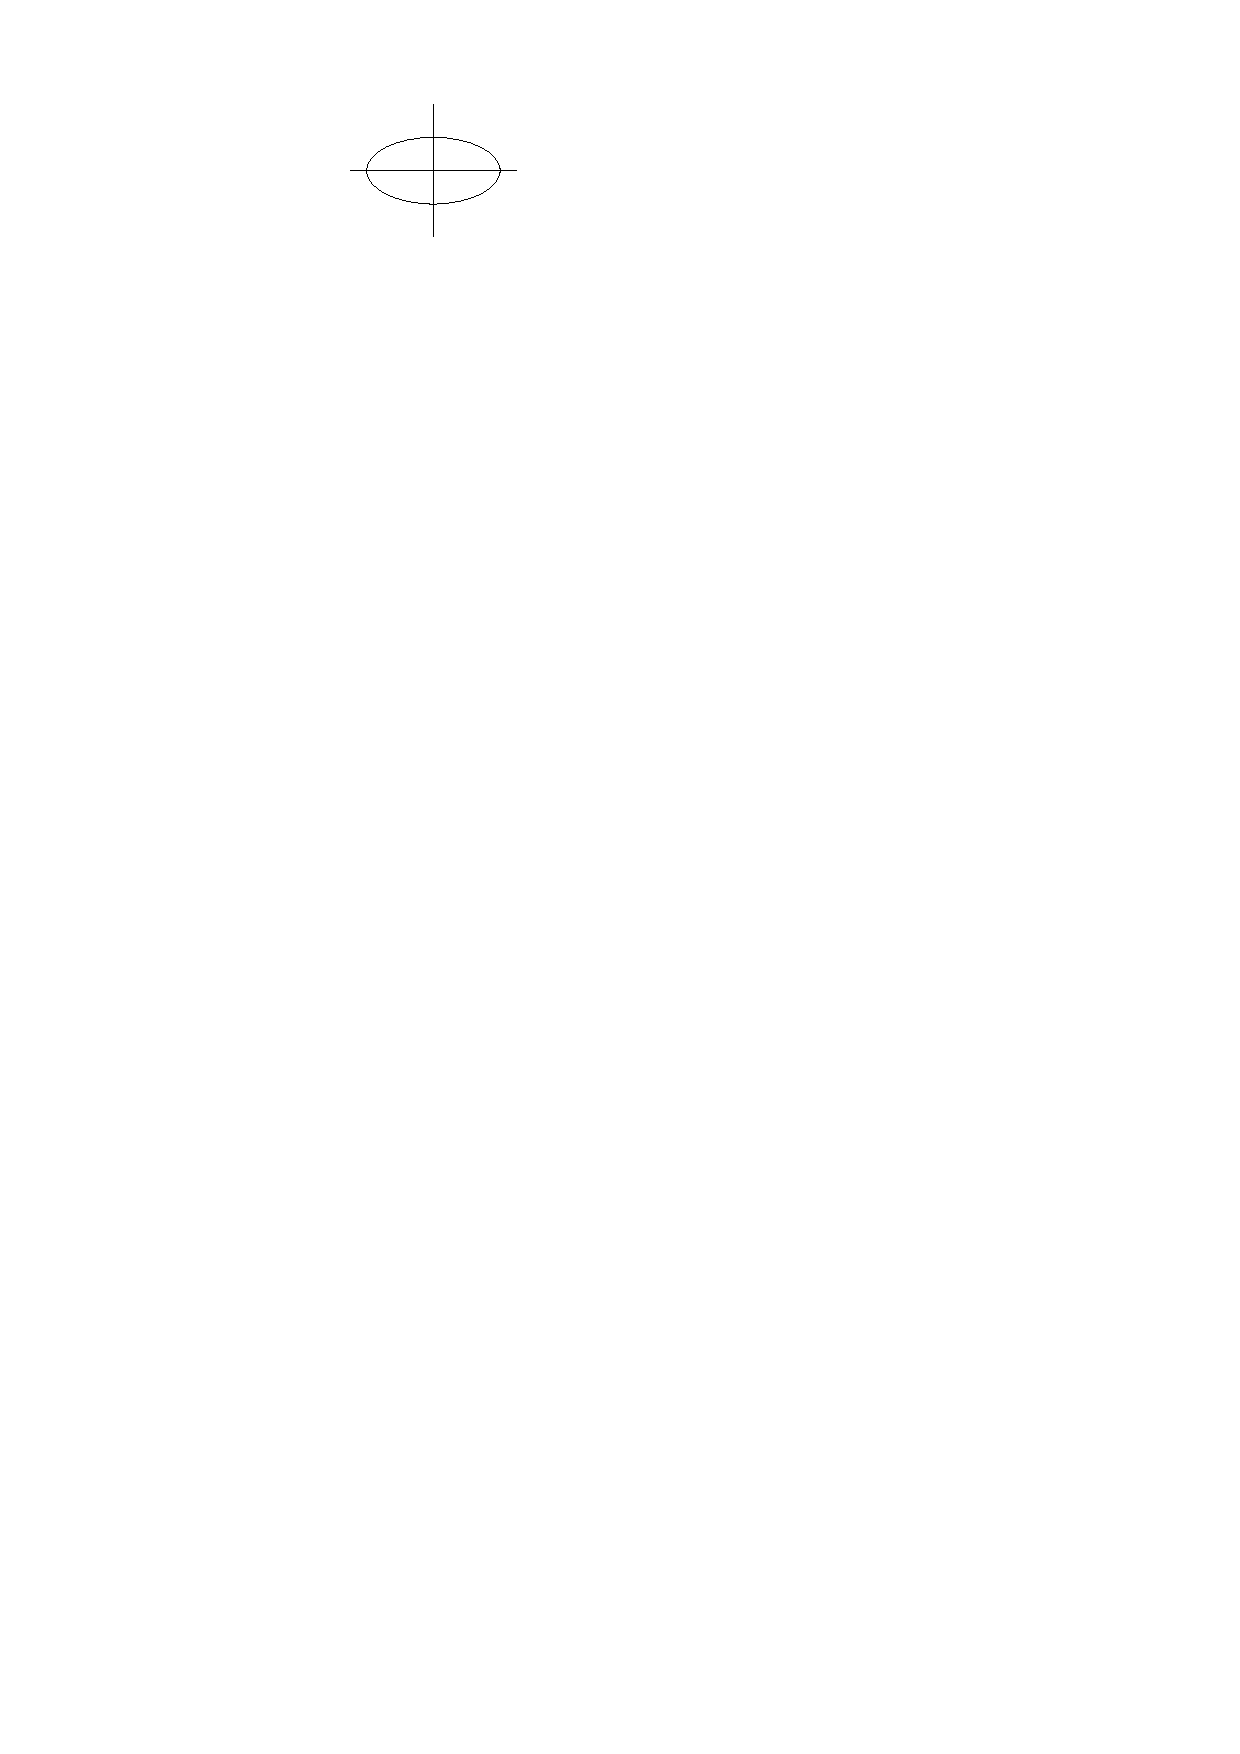
\includegraphics{figures/ueb3/aufgabe5a}
		\caption{Eine Ellipse.}
		\label{fig:ueb3_aufgabe5a}
	\end{figure}

	\item[b, i)] $\vec{r}(t) = (a \cos(\omega t), a \sin(\omega t), c t)$, oder getrennt: $x(t) = a \cos(\omega t)$, $y(t) = a \sin(\omega t)$ und $z(t) = ct$.
	 
	Das ist ein Kreis mit einem linearen "`displacement"' in der $z$-Achse; also eine Art Schraube.
	
	\item[b, ii)] Wir suchen $\Delta z = z(t_2) - z(t_1)$, wobei $x(t_1) = x(t_2)$ und $y(t_1) - y(t_2)$. Man nennt $\Delta z$ auch "`helicoid step"'.
	
	Einsetzen: $x(t_1) = \cos(\omega t_1)$, $x(t_2) = \cos(\omega t_2)$; also $x(t_1) = x(t_2)$ genau dann, wenn $\omega t_1 = \omega t_2 + 2 \pi n$ mit $n \in \mathbb{N}$. Also erfüllt für $\Delta t = \frac{2 \pi}{\omega}$ und Vielfache davon. Damit: $\Delta z = c (t_2 - t_1) = c \Delta t = \frac{2 \pi c}{\omega}$. $\frac{2 \pi}{\omega} =: T$ ist die Periode.
	
	\item[c)] Rechne 
	\begin{align*}
		\vec{v}(t) &= \msimplediff{\vec{r}}{t} = (-r \omega \sin(\omega t), r \omega \cos(\omega t), 0) \\
		\vec{a}(t) &= \msimplediff{\vec{v}}{t} = (-r \omega^2 \cos(\omega t), -r \omega^2 \sin(\omega t), 0) = -\omega^2 \vec{r}(t)
		\text{.}
	\end{align*}
	Siehe Abbildung \ref{fig:ueb3_aufgabe5c} für die Visualisierung der drei Vektoren.
	
	\begin{figure}[h]
		\centering
		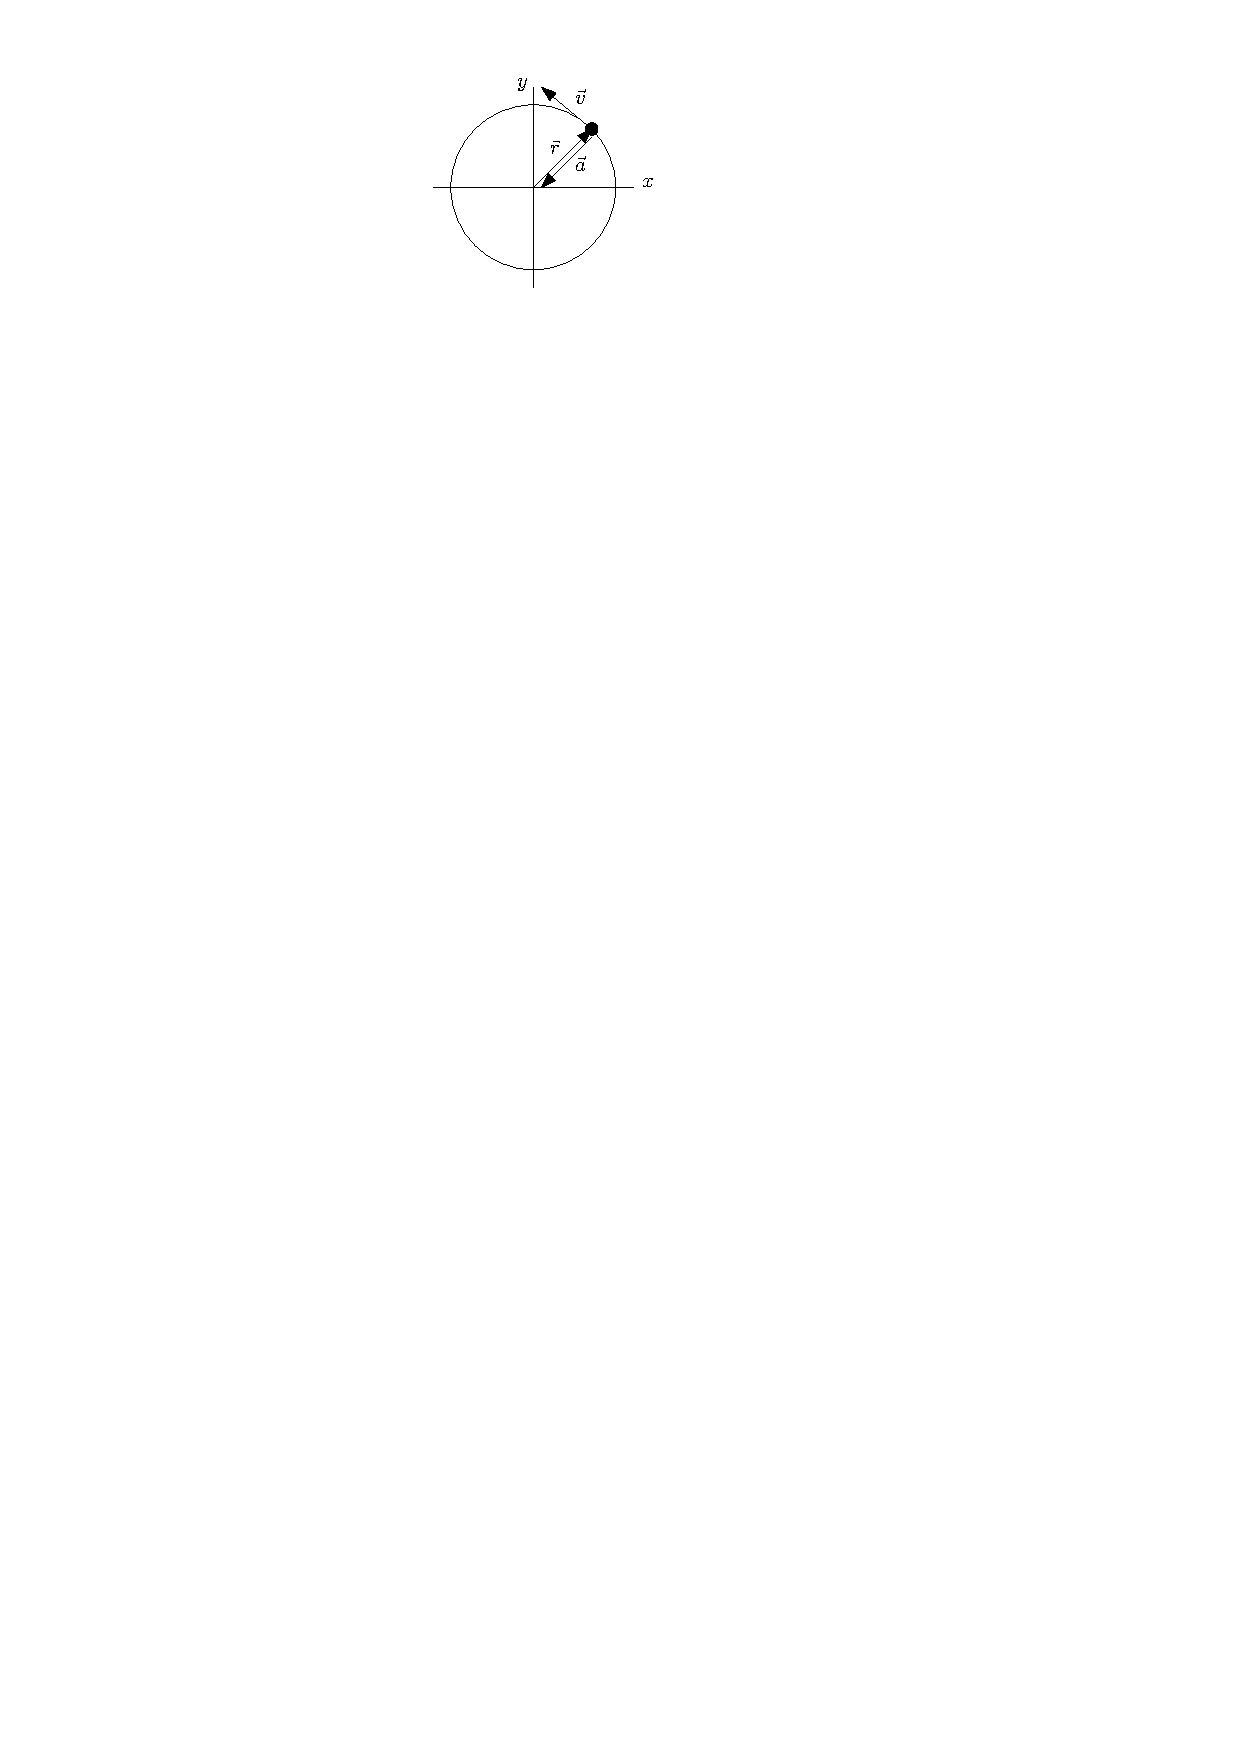
\includegraphics{figures/ueb3/aufgabe5c}
		\caption{Vektore $\vec{r}$, $\vec{v}$ und $\vec{a}$ bei Aufgabe 5c.}
		\label{fig:ueb3_aufgabe5c}
	\end{figure}
	
	Für die Kreisbahn muss nun gelten: $-G \frac{M_e m_s}{r^3} \vec{r} \overset{!}{=} -m_s \omega^2 \vec{r}$. Dass das $m_s$ auf beiden Seiten gleich ist, ist alles andere als trivial und führt auf Einstein zurück; aktuell ist uns das aber egal.
	
	Mit Kürzen erhalten wir
	\[
		-G \frac{M_e}{r^3} \overset{!}{=} -\omega^2 \quad \Rightarrow \quad \omega = \sqrt{ \frac{G M_e}{r} } \frac{1}{r}
		\text{.}
	\]
	
	Beobachtung: $T^2 \approx r^3$; das ist Kepler's Dritte Gesetz.
\end{description}

\section*{Aufgabe 6}

Siehe Abbildung \ref{fig:ueb3_aufgabe6} für eine Skizze. Es gilt $\vec{a} = \msimplediff{\vec{v}}{t}$, also $\mathrm{d} \vec{v} = \vec{a} \mathrm{d} t$. Das integrieren wir:
	\begin{align*}
		& \int_{\vec{v}_0}^{\vec{v}} \mathrm{d} \vec{v}' = \int_{t = 0}^{t} \vec{a} \mathrm{d} t' \\
		\Rightarrow &~ \vec{v} - \vec{v}_0 = (0, 0, -gt) \\
		\Rightarrow &~ \vec{v} = \vec{v}_0 + (0, 0, -gt) = (v \cos(\alpha), 0, v \sin(\alpha) - gt)
		\text{.}
	\end{align*}
	
	Das gleiche Spiel nochmal:
	\[
		\vec{r} = \msimplediff{\vec{v}}{t} 
		\quad \Rightarrow \quad \int_{\vec{r_0}}^{\vec{r}} \mathrm{d} \vec{r}' = \int_{t = 0}^t \vec{v} \mathrm{d} t'
		\quad \Rightarrow \quad \vec{r}(t) - \vec{r}_0 = (v \cos(\alpha t), 0, v \sin(\alpha t) - \frac{1}{2} g t^2)
	\]
	
	Oder getrennt geschrieben: $x(t) = v \cos(\alpha t)$, $y(t) = 0$ und $z(t) = v \sin(\alpha t) - \frac{1}{2} g t^2$. Beobachtung: $z(t)$ wird an zwei Punkten $0$: für $t = 0$ und für $t = \frac{2 v \sin(\alpha)}{g}$.
	
	\begin{figure}[h]
		\centering
		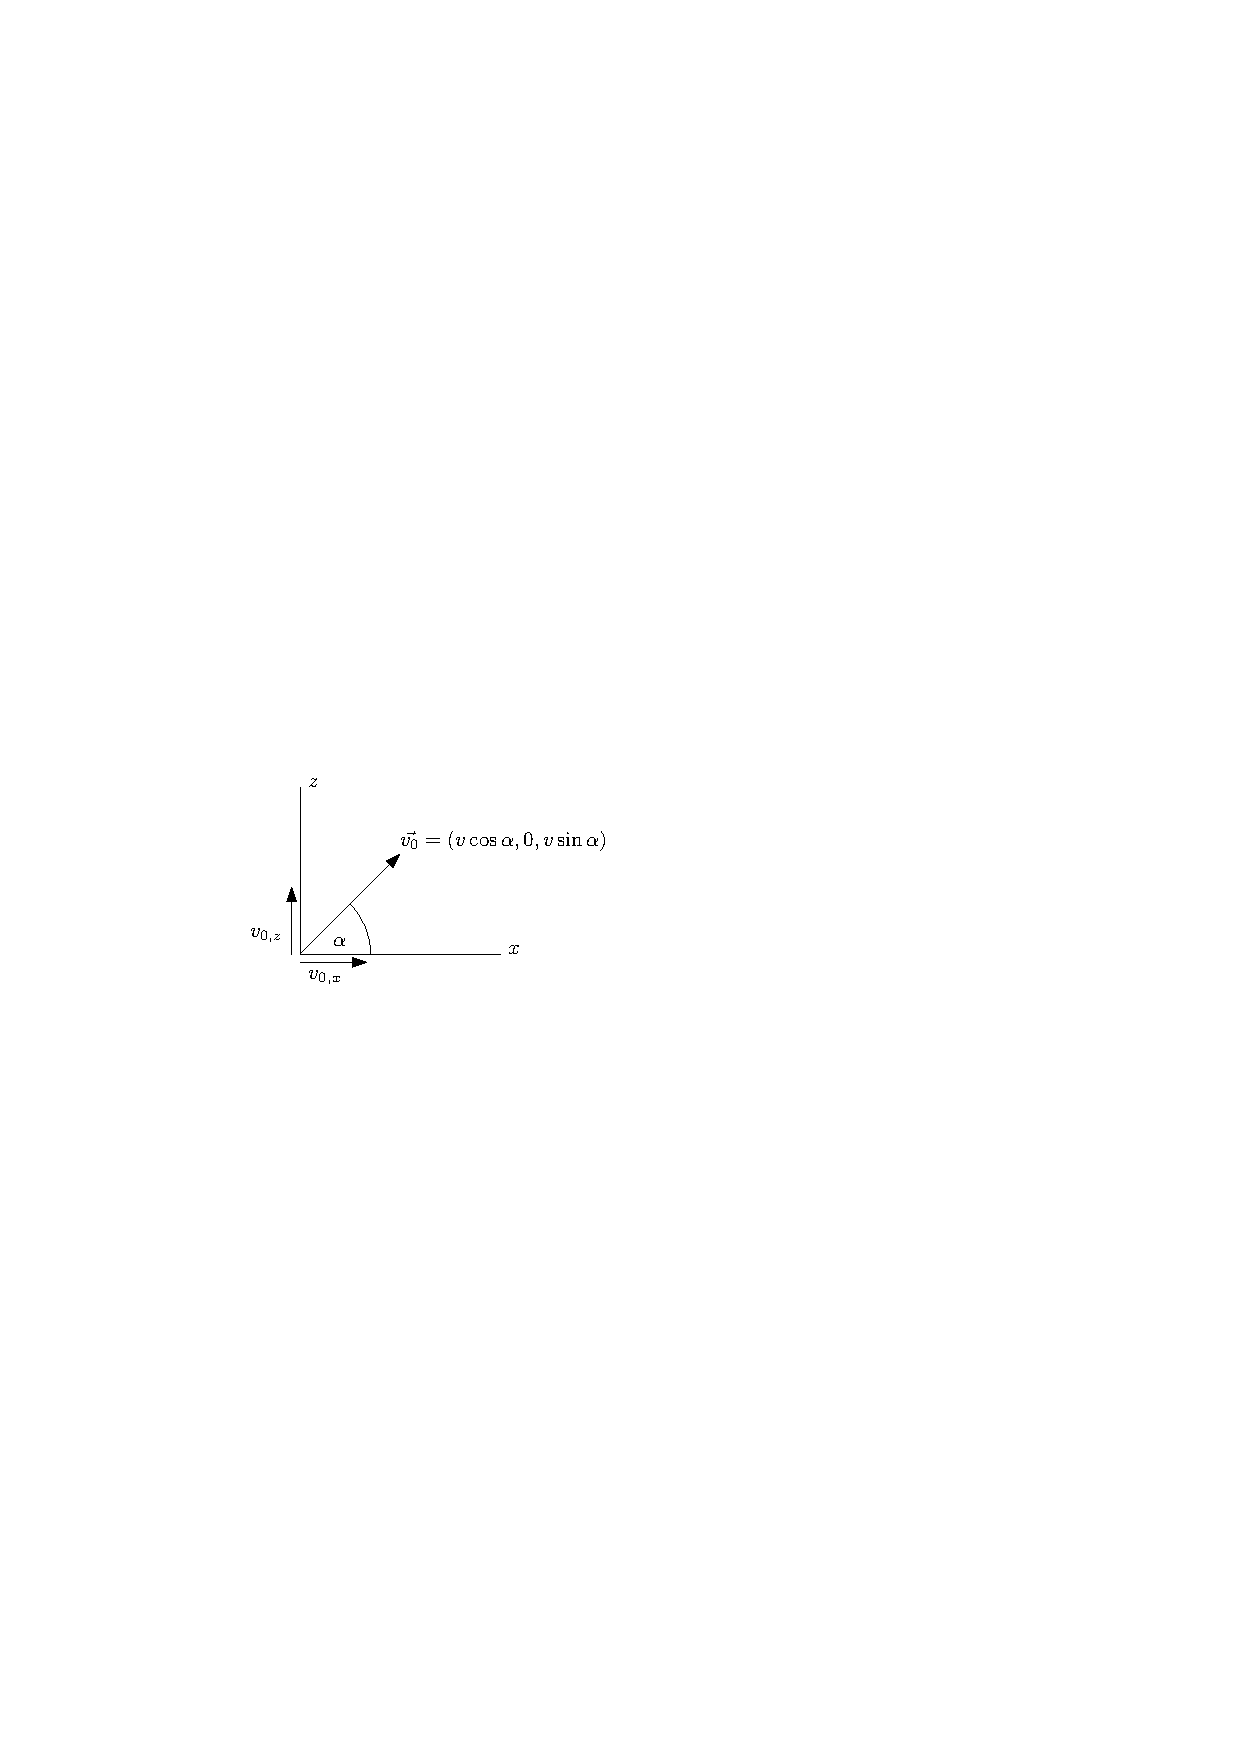
\includegraphics{figures/ueb3/aufgabe6}
		\caption{Eingangssituation in Aufgabe 6.}
		\label{fig:ueb3_aufgabe6}
	\end{figure}
	
	Aus der $x$-Gleichungen erhalten wir $t = \frac{x}{v \cos(\alpha)}$. Also $z(x) = x \tan(\alpha) - \frac{gx^2}{2 v^2 \cos^2(\alpha)}$. Das ist eine Parabel. Die Nullstellen von $z(x)$ sind $x = 0$ und $x = \frac{2 v^2 \sin(\alpha) \cos(\alpha)}{g} = v \cos(\alpha) \underbrace{\frac{2 v \sin(\alpha)}{g}}_{\text{Nullstelle von $z(t)$}}$.
	
	Für welches $\alpha'$ wird ist die Wurfweite maximal? Maximiere $x_{\text{reach}}(\alpha)$. Es gilt
	\[
		\msimplediff{x_{\text{reach}}(\alpha)}{\alpha} = \frac{2v^2}{g} (\cos^2(\alpha) \sin^2(\alpha)) = \frac{2 v^2}{g} \cos(2 \alpha)
		\text{.}
	\]
	Eine Nullstelle $\alpha'$ davon erfüllt $\cos(2 \alpha') = 0$, also $2 \alpha' = \frac{\pi}{2}$ und damit $\alpha' = \frac{\pi}{4}$.

\section*{Aufgabe 7}

Für eine Skizze siehe Abbildung \ref{fig:ueb3_aufgabe7}.

\begin{figure}[h]
	\centering
	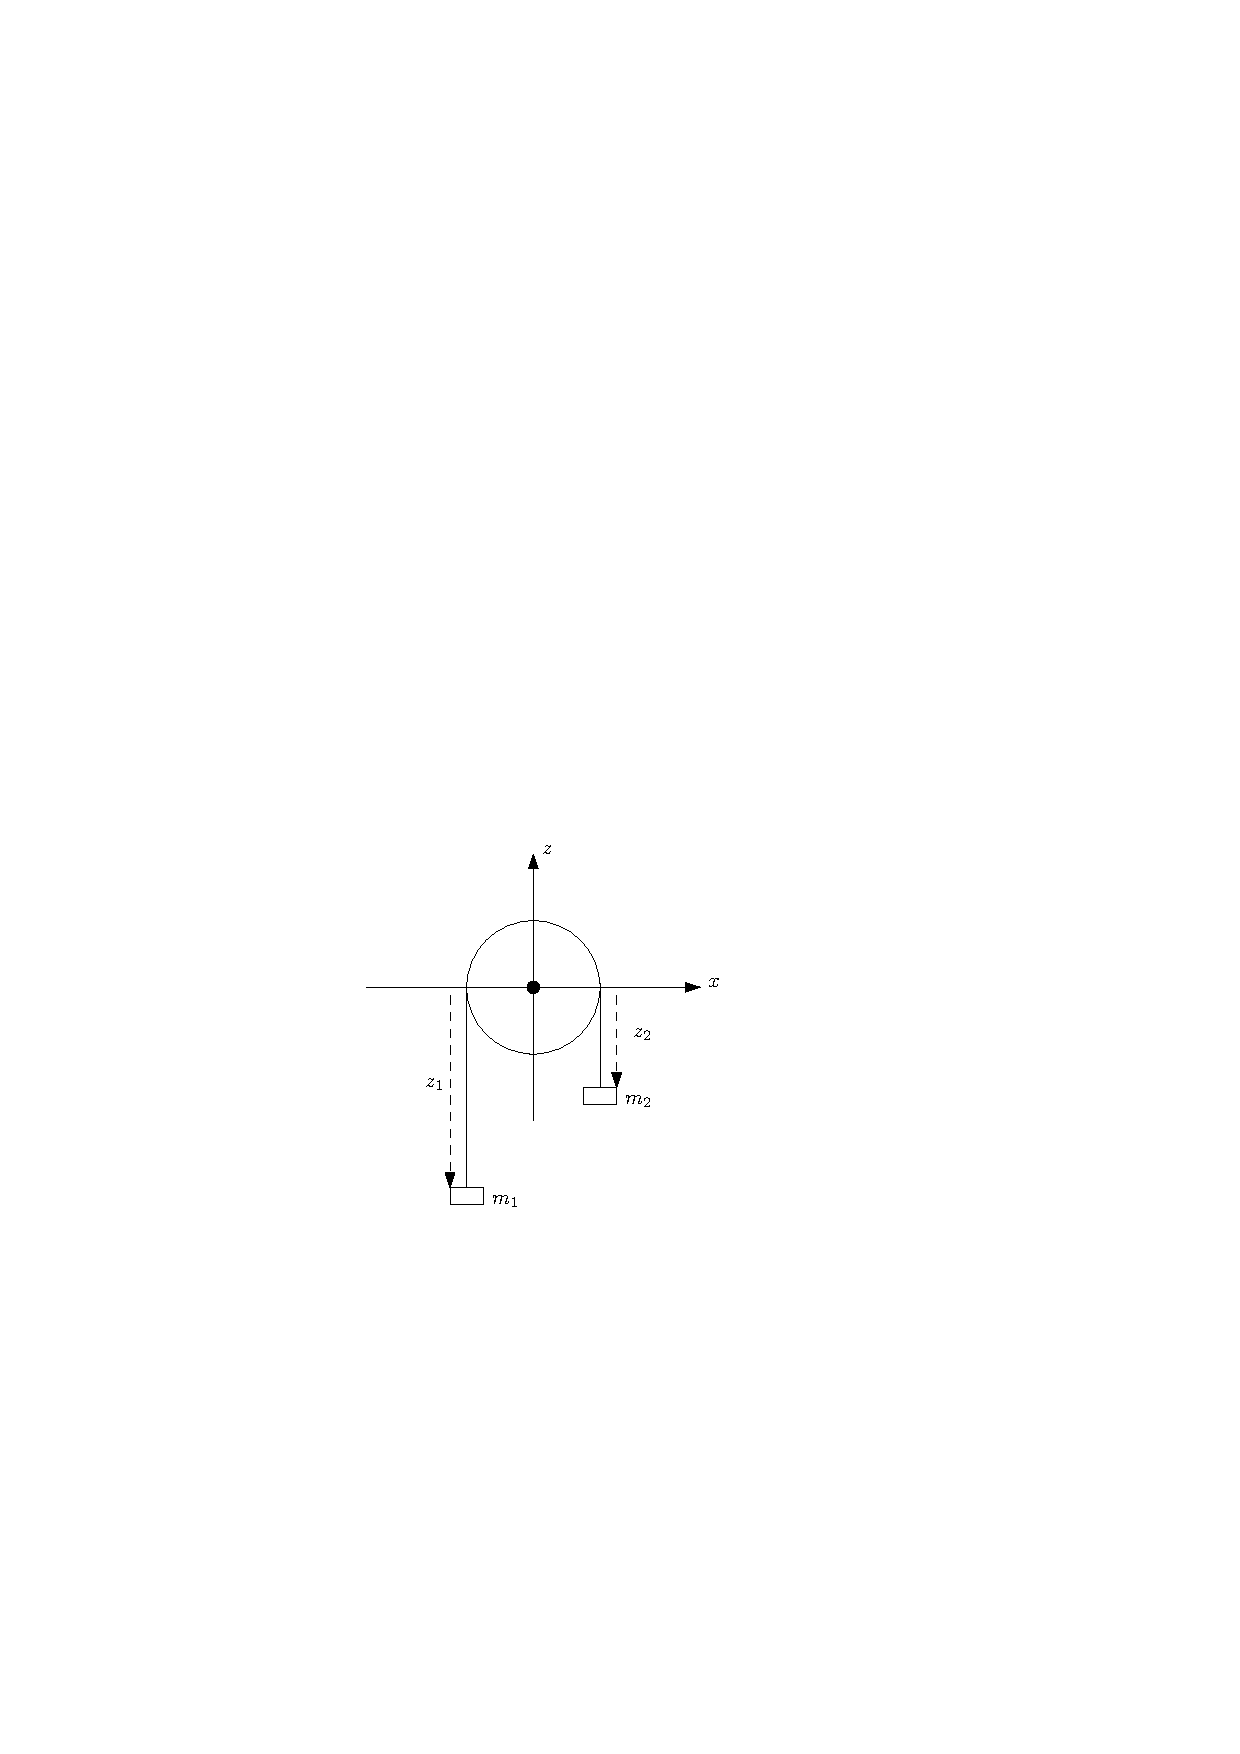
\includegraphics{figures/ueb3/aufgabe7}
	\caption{Die Massen $m_1$ und $m_2$ können sich nur vertikal bewegen.}
	\label{fig:ueb3_aufgabe7}
\end{figure}

Die generalisierten Koordinaten(?,\footnote{nur $(z_1, \dot(z)_1)$ sind generalisierte Koordinaten?}) sind $(z_1, z_2, \dot{z}_1, \dot{z}_2)$ und die Constraints sind Maximale Länge des Fadens, $l = \mabs{z_1} + \mabs{z_2} = -z_1 - z_2$.

Nun die Lagrange-Funktion aufstellen (beachte: $g < 0$, $z_2 = -z_1 - l$, $\dot{z}_2 = \dot{z}_1$): 
\begin{align*}
	L(z_1, z_2, \dot{z}_1, \dot{z}_2) 
	&= T - V = \sum_i T_i - V_i \\
	&= \frac{1}{2} m_1 \vec{z}_1^2 + \frac{1}{2} m_2 \dot{z}_2^2 + m_1 z_1 g + m_2 z_2 g \\
	&= \frac{1}{2} (m_1 + m_2) \dot{z}_1^2 + (m_1 - m_2) g z_1 - m_2 g l
	\text{.}
\end{align*}
Durch das Constraint konnten wir die Lagrange-Funktion also mit nur $(z_1, \dot{z}_1)$ statt $(z_1, z_2, \dot{z}_1, \dot{z}_2)$ ausdrücken.

Anders ausgedrückt: 2 Teilchen, die sich in 1D bewegen, haben zwei Grad Freiheit; das führt auf $4$ Koordinaten. Da wir aber ein Constraint haben, gibt es nur noch ein Grad Freiheit, für das wir nur noch ein Paar Koordinaten brauchen.

Nun muss gelten $\msimplediff{}{t} \frac{\partial L}{\partial \dot{z}_1} = \frac{\partial L}{\partial z_1}$, wobei
\begin{align*}
	\frac{\partial L}{\partial z_1} &= (m_1 - m_2) g, \\
	\msimplediff{}{t} \frac{\partial L}{\partial \dot{z}_1} &= (m_1 + m_2) \ddot{z}_1 
	\text{.}
\end{align*}
Also $(m_1 + m_2) \ddot{z}_1 = (m_1 - m_2) g$ und damit \fbox{$\ddot{z}_1 = g \frac{m_1 - m_2}{m_1 + m_2}$}.


	\chapter*{Übung 4}

\section*{Aufgabe 8}

Erinnerung: $\dot{x}(t) = \msimplediff{x(t)}{t}$ und $\ddot{x}(t) = \frac{\mathrm{d}^2 x(t)}{\mathrm{d} t^2}$.

Zu lösende Gleichung:
\[
	\ddot{x}(t) = -\frac{k}{m} x(t)
	\text{.}
\]

Ansatz: $x(t) = c_\lambda e^{\lambda t}$; also $\dot{x}(t) = \lambda c_\lambda e^{\lambda t}$ und $\ddot{x}(t) = \lambda^2 c_\lambda e^{\lambda t}$. Das in die zu lösende Gleichung einsetzen:
\[
	\lambda^2 c_\lambda c^{\lambda t} = -\frac{k}{m} c_\lambda e^{\lambda t}
	\quad \Longleftrightarrow \quad
	\lambda^2 = -\frac{k}{m}
	\quad \Longrightarrow \quad
	\lambda = \pm i \sqrt{\frac{k}{m}}
	\text{.}
\]

Die allgemeine Lösung lautet also: $x(t) = c_1 e^{it \sqrt{k / m}} + c_2 e^{-it \sqrt{k / m}}$ und die Ableitung davn ist: $\dot{x}(t) = \sqrt{\frac{k}{m}} \left( c_1 e^{it \sqrt{k / m}} - c_2 e^{-it \sqrt{k / m}} \right)$.

Nun sollen die Konstanten $c_1$ und $c_2$ bestimmt werden. Dazu die Anfangsbedingungen einsetzen:
\begin{align*}
	x_0 &\overset{!}{=} x(t = 0) = c_1 + c_2,	 \\
	v_0 &\overset{!}{=} \dot{x}(t = 0) = i \sqrt{\frac{k}{m}} (c_1 - c_2)
	\text{.}
\end{align*}
Das führt auf $c_1 = \frac{1}{2} \left( x_0 + \frac{1}{i} \sqrt{\frac{m}{k}} v_0 \right)$ und $c_2 = \frac{1}{2} \left( x_0 - \frac{1}{i} \sqrt{\frac{m}{k}} v_0 \right)$. Eingesetzt ergibt das die Lösung
\[
	x(t) = \frac{1}{2} x_0 \left( e^{it \sqrt{k / m}} + e^{-it \sqrt{k / m}} \right)
	+ \frac{1}{2i} \sqrt{\frac{m}{k}} v_0 \left( e^{it \sqrt{k / m}} - e^{-it \sqrt{k / m}} \right)
	\text{.}
\]

Um den Term weiter zu vereinfachen, verwende $\frac{k}{m} = \omega^2$. Das führt auf auf die vereinfachte Lösung
\[
	x(t) = x_0 \cos(\omega t) + \frac{v_0}{\omega} \sin(\omega t)
	\text{.}
\]

Zuletzt berechnen wir die Energie, wobei $\dot{x}(t) = -x_0 \omega \sin(\omega t) + v_0 \omega \cos(\omega t)$:
\begin{align*}
	E &= T + V = \frac{1}{2} m \dot{x}^2 + \frac{1}{2} k x^2	 = \frac{1}{2} m \left( \dot{x}^2(t) + \omega^2 x^2(t) \right) \\
	&= \dots = \frac{1}{2} m \left( v_0^2 + \omega^2 x_0^2 \right) = \frac{1}{2} m v_0^2 + \frac{1}{2} k x_0^2
	\text{.}
\end{align*}

\section*{Aufgabe 9}
Siehe Abbildung \ref{fig:ueb4_aufgabe9} für eine Skizze mit den Variablen.

\begin{figure}[h]
	\centering
	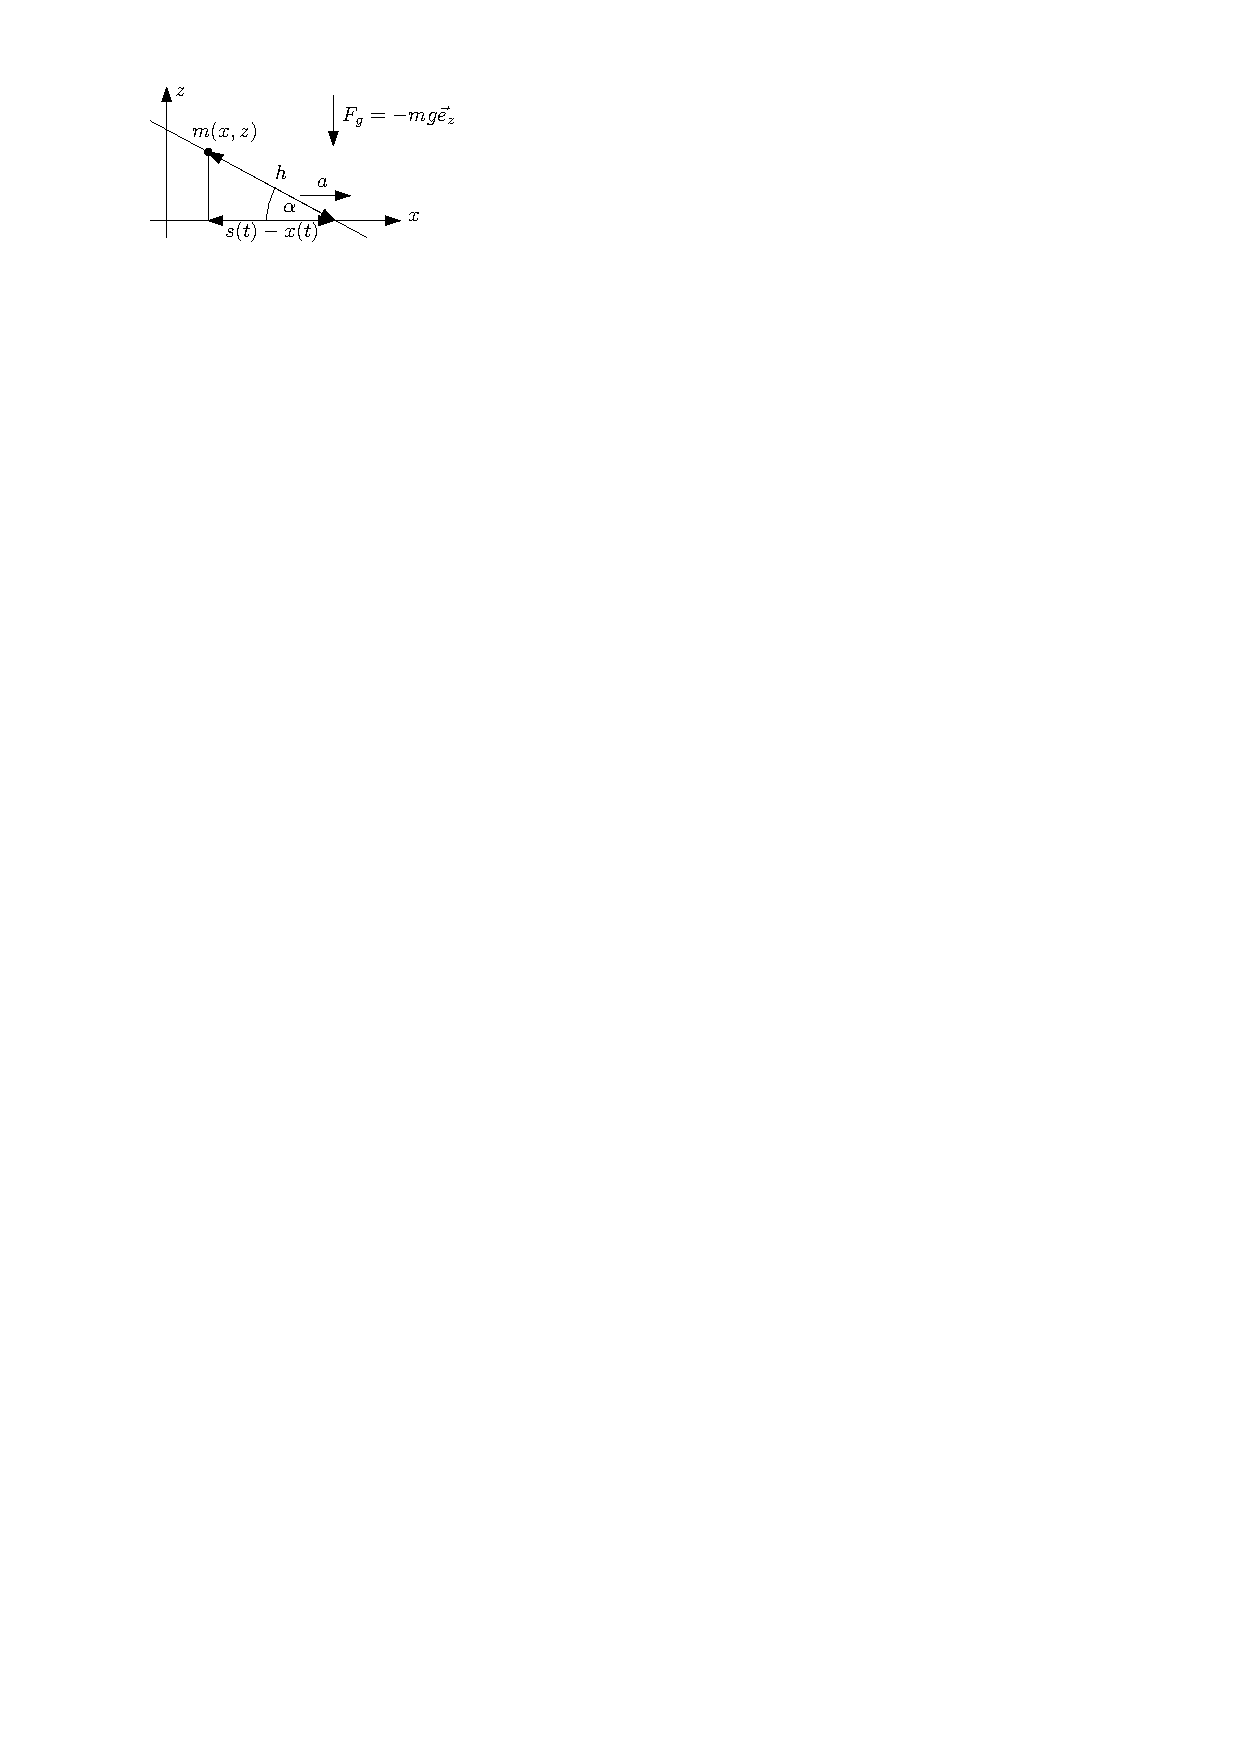
\includegraphics[scale=1.5]{figures/ueb4/aufgabe9}
	\caption{Skizze für die Variablen von Aufgabe 9.}
	\label{fig:ueb4_aufgabe9}
\end{figure}

Es gilt $\sin \alpha = \frac{z(t)}{h}$ und $\cos \alpha = \frac{s(t) - x(t)}{h}$, also
\[
	\frac{z(t)}{\sin \alpha} = \frac{s(t) - x(t)}{\cos \alpha}
	\quad \Longleftrightarrow \quad 
	z(t) \cos(\alpha) = (s(t) - x(t)) \sin \alpha
	\text{.}
\]

Die Zwangsbedingung ist damit $A(x, z, t) = \left( x(t - \underbrace{\frac{1}{2} a t^2}_{= s(t)} \right) \sin(\alpha) + z(t) \cos(\alpha) \overset{!}{=} 0$.

Die Formel für die Zwangskräfte lautet $Z_i(x, z, t) = \lambda \frac{\partial A(x, z, t)}{\partial x_i}$. Damit berechnen wir:
\[
	\mvec{Z_x \\ Z_z} 
	= \mvec{\lambda \frac{\partial A(\cdot)}{\partial x} \\ \lambda \frac{\partial A(\cdot)}{\partial z}}
	= \lambda \mvec{\sin(\alpha) \\ \cos(\alpha)}
	\text{.}
\]

Wie berechnen wir die Lagrange-Multiplier $\lambda$? Ansatz:
\[
	m \mvec{\ddot{x}(t) \\ \ddot{z}(t)} 
	= \mvec{F_x + Z_x \\ F_z + Z_z}
	= \mvec{0 + \lambda \sin(\alpha) \\ -mg + \lambda \cos(\alpha)}
\]
Weiter brauchen wir: 
\begin{align*}
	\frac{\partial A(\cdot)}{\partial t} &= \left( \dot{x}(t) - at \right) \sin(\alpha) + \dot{z}(t) \cos(\alpha) \overset{!}{=} 0 \text{ und } \\
	\frac{\partial A(\cdot)}{\partial t^2} &= \left( \ddot{x}(t) - a \right) \sin(\alpha) + \ddot{z}(t) \cos(\alpha) \overset{!}{=} 0
	\text{.}
\end{align*}
Daraus gewinnen wir $\ddot{z}(t) = - (\ddot{x}(t) - a) \tan(\alpha)$, das wir in obige Kraftgleichung geteilt durch $m$ einsetzen:
\[
	\mvec{\ddot{x}(t) \\ -(\ddot{x}(t) - a) \tan(\alpha)}
	= \mvec{ \frac{\lambda}{m} \sin(\alpha) \\ -g + \frac{\lambda}{m} \cos(\alpha) }
	\quad \Longleftrightarrow \quad 
	\mvec{\ddot{x}(t) \\ \ddot{x}(t)} = \mvec{ \frac{\lambda}{m} \sin(\alpha) \\ a + g \cot(\alpha) - \frac{\lambda}{m}  \cos(\alpha) \cot(\alpha) }
	\text{.}
\]

Nun können wir das $\lambda$ bestimmen, denn es folgt die Bedingung
\begin{align*}
	& \frac{\lambda}{m} \sin(\alpha) = a + g \cot(\alpha) - \frac{\lambda}{m} \cos(\alpha) \cot(\alpha) \\
	\Longleftrightarrow~ & \frac{\lambda}{m} \left( \sin(\alpha) + \frac{\cos^2(\alpha)}{\sin(\alpha)} \right) = a + g \frac{\cos(\alpha)}{\sin(\alpha)} \\
	\Longleftrightarrow~ & \frac{\lambda}{m} \frac{1}{\sin(\alpha)} = a + g \frac{\cos(\alpha)}{\sin(\alpha)} \\
	\Longleftrightarrow~ & \lambda = m ( a \sin(\alpha) + g \cos(\alpha) )	
\end{align*}

Das wieder in die Kraftgleichung geteilt durch $m$ einsetzen:
\[
	\mvec{\ddot{x}(t) \\ \ddot{z}(t)} 
	= \mvec{ (a \sin(\alpha) + g \cos(\alpha)) \sin(\alpha) \\ - g + (a \sin(\alpha) + g \cos(\alpha)) \cos(\alpha)}
	\text{.}
\]

Anfangsbedingungen: $\dot{x}(t = 0) = v_0$ und $x(t = 0) = x_0$. Damit noch $x(t)$ berechnen: 
\begin{align*}
	\dot{x}(t) 
	&= \int_0^t \ddot{x}(t') \md t' + \underbrace{\dot{x}(t = 0)}{= v_0}
	= t \sin(\alpha) (a \sin(\alpha) + g \cos(\alpha) + v_0 \\
	x(t)
	&= \int_0^t \dot{x}(t') \md t' + \underbrace{x(t = 0)}{= x_0}
	= \frac{1}{2} t^2 \sin(\alpha) (a \sin(\alpha) + g \cos(\alpha)) + v_0 t + x_0
\end{align*}
Das fehlende $z(t)$ kann man nun aus $A(x, z, t) = 0$ berechnen:
\[
	z(t) = \frac{1}{2} t^2 \sin(\alpha) (a \cos(\alpha) - g \sin(\alpha)) - (v_0 t + x_0) \tan(\alpha)
	\text{.}
\]

\section*{Aufgabe 10}

Koordinaten sind gegeben durch $\vec{x} = r \mvec{\sin \theta \cos \phi \\ \sin \theta \sin \phi \\ \cos \theta} = \mvec{x \\ y \\ z}$.

Zunächst die Richtungsvektoren berechnen: 
\begin{align*}
	\vec{k}_r &= \frac{\partial \vec{x}}{\partial r} = \mvec{ \sin \theta \cos \phi \\ \sin \theta \sin \phi \\ \cos \theta}, \\
	\vec{k}_\theta &= \frac{\partial \vec{x}}{\partial \theta} = r \mvec{\cos \theta \cos \phi \\ \cos \theta \sin \phi \\ -r \sin \theta}, \\
	\vec{k}_\phi &= \frac{\partial \vec{x}}{\partial \phi} = r \sin \theta \mvec{ - \sin \phi \\ \cos \phi \\ 0}
	\text{.}
\end{align*}

Für die Einheitsvektoren berechnen wir die Länge der Vektoren:
\begin{align*}
	\mabs{\vec{k}_r} &= \sqrt{\vec{k}_r^2} = \sqrt{\sin^2 \theta \cos^2 \phi + \sin^2 \theta \sin^2 \phi + \cos^2 \theta} = \sqrt{\underbrace{\sin^2 \theta \underbrace{(\cos^2 \phi + \sin^2 \phi)}_{ = 1} + \cos^2 \theta}_{= 1}} = 1, \\
	\mabs{\vec{k}_\theta} &= \sqrt{\vec{k}_\theta^2} = \dots = \sqrt{r^2} = r, \\
	\mabs{\vec{k}_\phi} &= \sqrt{\vec{k}_\phi^2} = \sqrt{r^2 \sin^2 \theta (\sin^2 \phi + \cos^2 \phi)} = r \sin \theta
	\text{.}
\end{align*}
Die Einheitsvektoren sind also:
\[
	\vec{e}_r = \mvec{\sin \theta \cos \phi \\ \sin \theta \sin \phi \\ \cos \theta},
	\quad 
	\vec{e}_\theta = \mvec{\cos \theta \cos \phi \\ \cos \theta \sin \phi \\ - \sin \theta},
	\quad 
	\vec{e}_\phi = \mvec{- \sin \phi \\ \cos \phi \\ 0}
	\text{.}
\]

Nun gilt für die zeitliche Ableitung von $x$:
\[
	\mdotvec{x}(t) 
	= \msimplediff{\vec{x}}{t} 
	= \msimplediff{r}{t} \frac{\partial \vec{x}}{\partial r}
	+ \msimplediff{\theta}{t} \frac{\partial \vec{x}}{\partial \theta} 
	+ \msimplediff{\phi}{t} \frac{\partial \vec{x}}{\partial \phi}
	= \dot{r} \vec{e}_r + \dot{\theta} r \vec{e}_\theta + \dot{\phi} r \sin \theta \vec{e}_\phi
	\text{.}
\]

Damit kann man die kinetische Energie wie folgt schreiben:
\[
	T = \frac{1}{2} m \mdotvec{x}^2 = \frac{1}{2} m \left( \dot{r}^2 + r^2 \dot{\theta}^2 + r^2 \sin^2 \theta \dot{\phi}^2 \right)
	\text{.}
\]

Jetzt können wir die Lagrange-Funktion aufschreiben als 
\[
	\mathcal{L} = T - V = \frac{1}{2} m \left( \dot{r}^2 + r^2 \dot{\theta}^2 + r^2 \sin^2 \theta \dot{\phi}^2 \right) - V(r, t)
	\text{.}
\]

Die Lagrange-Funktion hängt also nicht explizit von $\phi$ ab. Also ist $\phi$ eine zyklische Koordinate. Denn eine Koordinate ist zyklisch, wenn $\frac{\partial \mathcal{L}}{\partial \phi} = 0 = \msimplediff{}{} \frac{\partial \mathcal{L}}{\partial \phi}$.

Der Impuls 
\[
	P \phi = \frac{\partial \mathcal{L}}{\partial \dot{\phi}} = mr^2 \sin^2 \theta \dot{\phi} \neq 0
\]
ist daher konstant, erhalten. In diesem Fall ist der Drehimpuls also erhalten.

\textbf{Anmerkung:} Es gilt
\[
	\frac{\partial L}{\partial q} = \msimplediff{}{t} \frac{\partial L}{\partial \dot{q}}
	\text{.}
\]
Wenn jetzt $\frac{\partial L}{\partial q} = 0$, dann ist auch $\msimplediff{}{t} \left( \frac{\partial L}{\partial \dot{q}} \right) = \msimplediff{}{t} Pp = 0$ (also zyklisch, wenn $Pp \neq 0$).
	\chapter{Übung 5}

\section*{Aufgabe 11}

Siehe Abbildung \ref{fig:ueb5_aufgabe11} für eine Skizze mit den Variablen.

\begin{figure}[h]
	\centering
	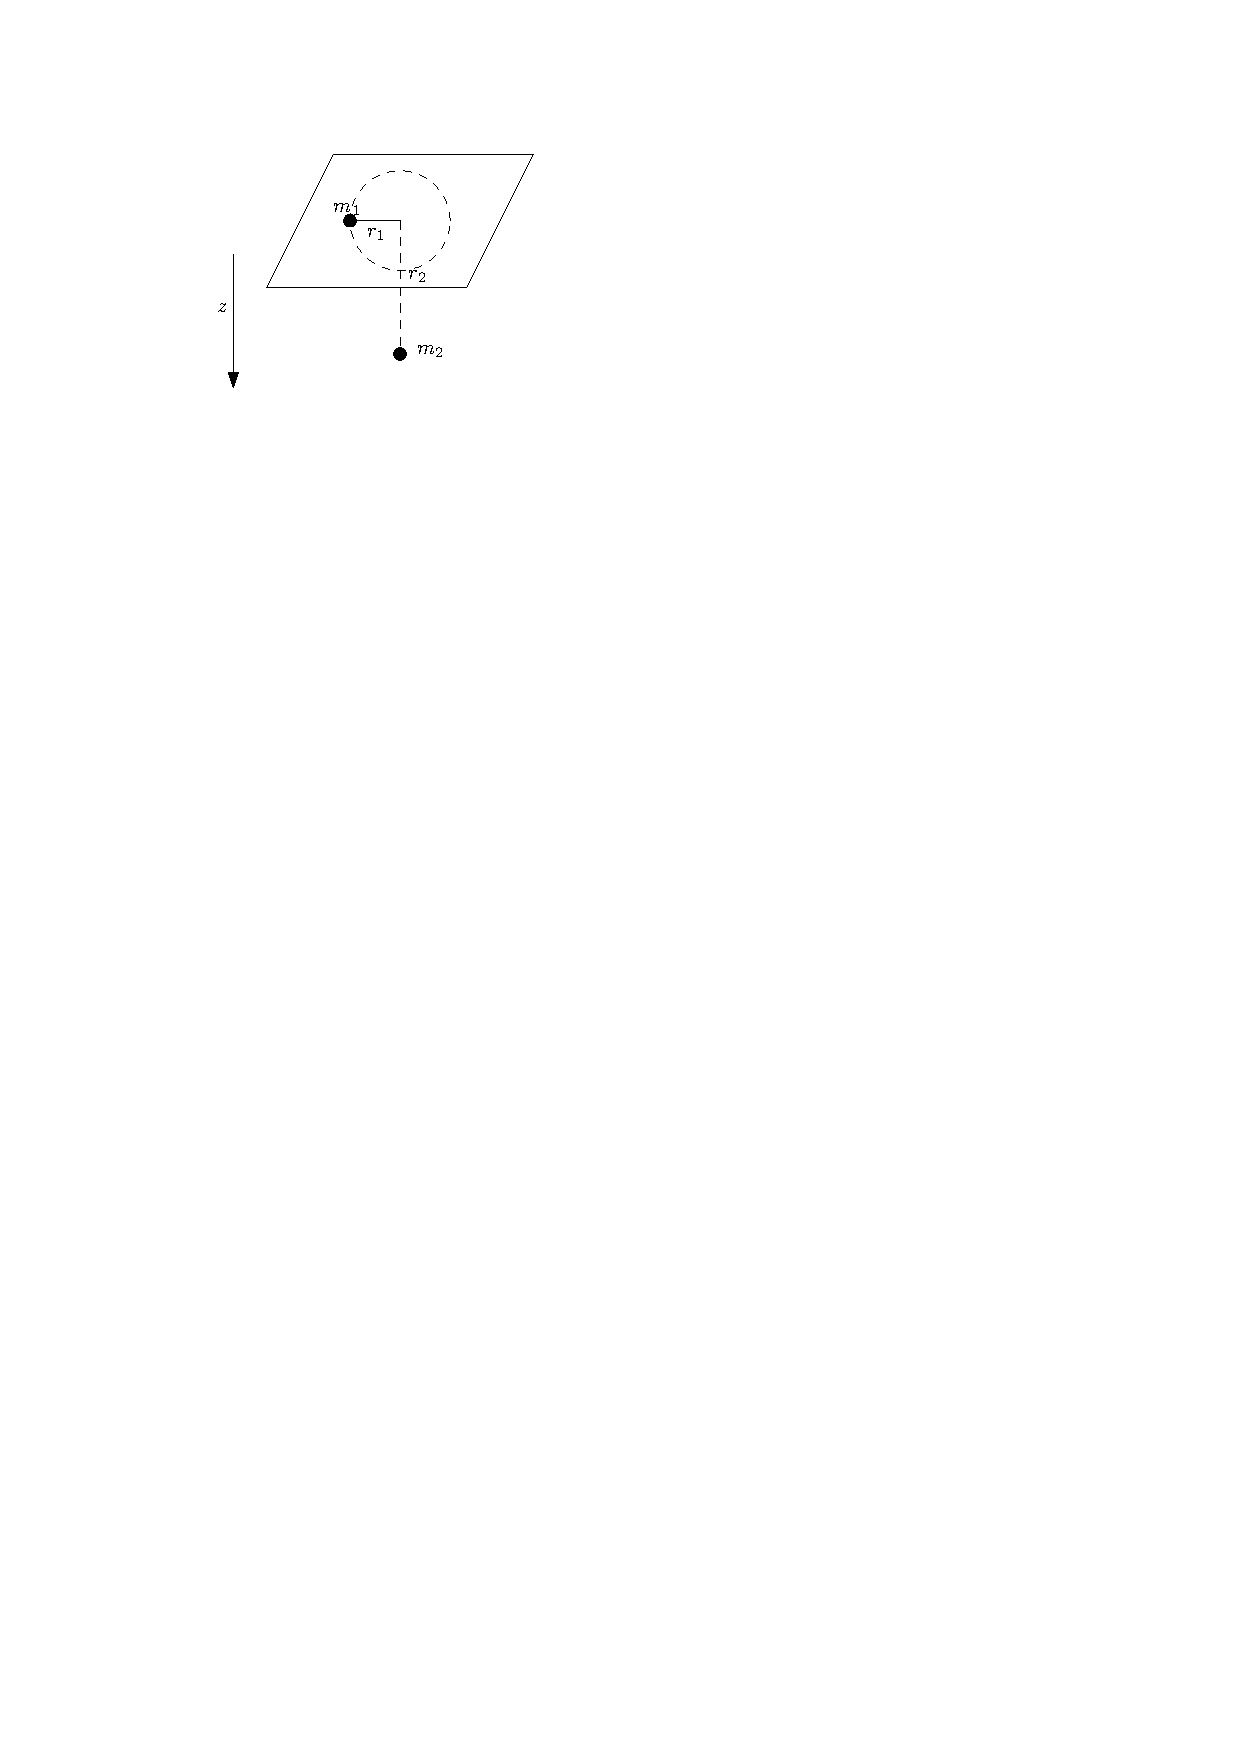
\includegraphics{figures/ueb5/aufgabe11}
	\label{fig:ueb5_aufgabe11}
	\chapter{Skizze von Aufgabe 11. Die Koordinate $z$ zeigt nach unten.}
\end{figure}

Wir wählen als Koordinaten:
\[
	\vec{x}_1 = \mvec{ \cos \phi_1 r_1 \\ \sin \phi_1 r_1 \\ z_1} 
	\quad \text{ und } \quad 
	\vec{x}_2 = r_2 \mvec{ \sin \theta_2 \cos \phi_2 \\ \sin \theta_2 \sin \phi_2 \\ \cos \theta_2 }
	\text{.}
\]

Also $F_g = m g \vec{e}_z = - \vec{\nabla} V_g$ mit $V_g = - m g z$ (auf Vorzeichen achten).

Die Länge vom Seil ist $l = r_1 + r_2$. Also Zwangsbedingung: $A = r_1 + r_2 - l = 0$ und $z_1 = const$. Wähle $z_1 = 0$, dann: $V_{g, 1} = - m_1 g \cdot 0 = 0$.

Damit ist $T_1 = \frac{1}{2} m_1 (\dot{x}_1^2 + \dot{y}_1^2)$, wobei 
\begin{align*}
	\dot{x}_1 &= \dot{r}_1 \cos \phi_1 - r_1 \dot{\phi}_1 \sin \phi_1 \text{ und} \\
	\dot{y}_1 &= \dot{r}_1 \sin \phi_1 + r_1 \dot{\phi}_1 \cos \phi_1 
	\text{.}	
\end{align*}

Also eingesetzt (Rechnung analog zu Aufgabe 10): $T_1 = \frac{1}{2} m_1 \left( \dot{r}_1^2 + r_1^2 \dot{\phi}_1^2 \right)$. Weiterhin 
\[
	T_2 \overset{\text{Aufg. 10}}{=} \frac{1}{2} m_2 \left( \dot{r}_1^2 + r_2^2 \dot{\theta})_2^2 + r_2^2 \dot{\phi}_2^2 \sin^2 \theta_2 \right)
	\text{.}
\]

Ingesamt folgt die Lagrange-Funktion, wobei $r_2 = l - r_1$ und $\dot{r}_2 = \dot{r}_1$ genutzt wird:
\begin{align*}
	L 
	&= T_1 + T_2 - V_1 - V_2 \\
	&= \frac{1}{2} m_1 \left( \dot{r}_1^2 + r_1^2 \dot{\phi}_1^2 \right)
	+ \frac{1}{2} m_2 \left( \dot{r}_2^2 + r_2 ^2 \dot{\theta}_2^2 + r_2^2 \dot{\phi}_2^2 \sin^2 \theta_2 \right)
	+ m g r_2 \cos \theta_2 \\
	&= \frac{1}{2} (m_1 + m_2) \dot{r}_1^2 
	+ \frac{1}{2} m_1 r_1^2 \dot{\phi}_1^2
	+ \frac{1}{2} (l - r_1)^2 (\dot{\theta}_2^2 + \dot{\phi}_2^2 \sin^2 \theta_2)
	+ m_2 g (l - r_1) \cos \theta_2
	\text{.}
\end{align*}

Was sind die zyklischen Koordinaten? Die müssen die Bedingung
\[
	\frac{\partial L}{\partial q_i} = 0 
	\quad \text{ und } \quad 
	\frac{\partial L}{\partial \dot{q}_i} \neq 0
\]
erfüllen.

Erhalten sind 
\begin{align*}
	P \phi_1 &= \frac{\partial L}{\partial \dot{\phi}_1} = m_1 r_1^2 \dot{\phi}_1 \text{ und } \\
	P \phi_2 &= \frac{\partial L}{\partial \dot{\phi}_2} = m_2 (l - r_1)^2 \sin^2 \theta_2 \dot{\phi}_2
	\text{.}
\end{align*}

Jetzt Einschränkung: $\phi_2 = \theta_2 = 0$. Damit vereinfacht sich die Lagrange-Funktion zu 
\[
	L = \frac{1}{2} (m_1 + m_2) \dot{r}_1^2 + \frac{1}{2} m_1 r_1^2 \dot{\phi}_1^2 + m_2 g (l - r_1) = L(r_1, \phi_1)
	\text{.}
\]	
Damit bestimmen wir die Lagrange-Gleichungen:
\begin{align*}
	& \frac{\partial L}{\partial r_1} = \msimplediff{}{t} \frac{\partial L}{\partial \dot{r}_1} \\
	\Longrightarrow~ & m_1 r_1 \dot{\phi}_1^2 - m_2 g = \msimplediff{}{t} \left( (m_1 + m_2) \dot{r}_1 \right) = (m_1 + m_2) \ddot{r}_1 \\
	\Longrightarrow~ & \ddot{r}_1 = \frac{1}{m_1 + m_2} \left( m_1 r_1 \dot{\phi}_1^2 - m_2 g \right) \\
	& \frac{\partial L}{\partial \phi_1} = \msimplediff{}{t} \frac{\partial L}{\partial \dot{\phi}} \\
	\Longrightarrow~ & 0 = \msimplediff{}{t} \left( m_1 r_1^2 \dot{\phi}_1 \right) = 2 m_1 \dot{r}_1 r_1 \dot{\phi}_1 + m_1 r_1^2 \ddot{\phi}_1 \\
	\Longrightarrow~ & \ddot{\phi}_1 = - \frac{2}{r_1} \dot{r}_1 \dot{\phi}_1
	\text{.}
\end{align*}

\section*{Aufgabe 12}

Für eine Skizze mit den Variablen siehe Abbildung \ref{fig:ueb5_aufgabe12}.

\begin{figure}
	\centering
	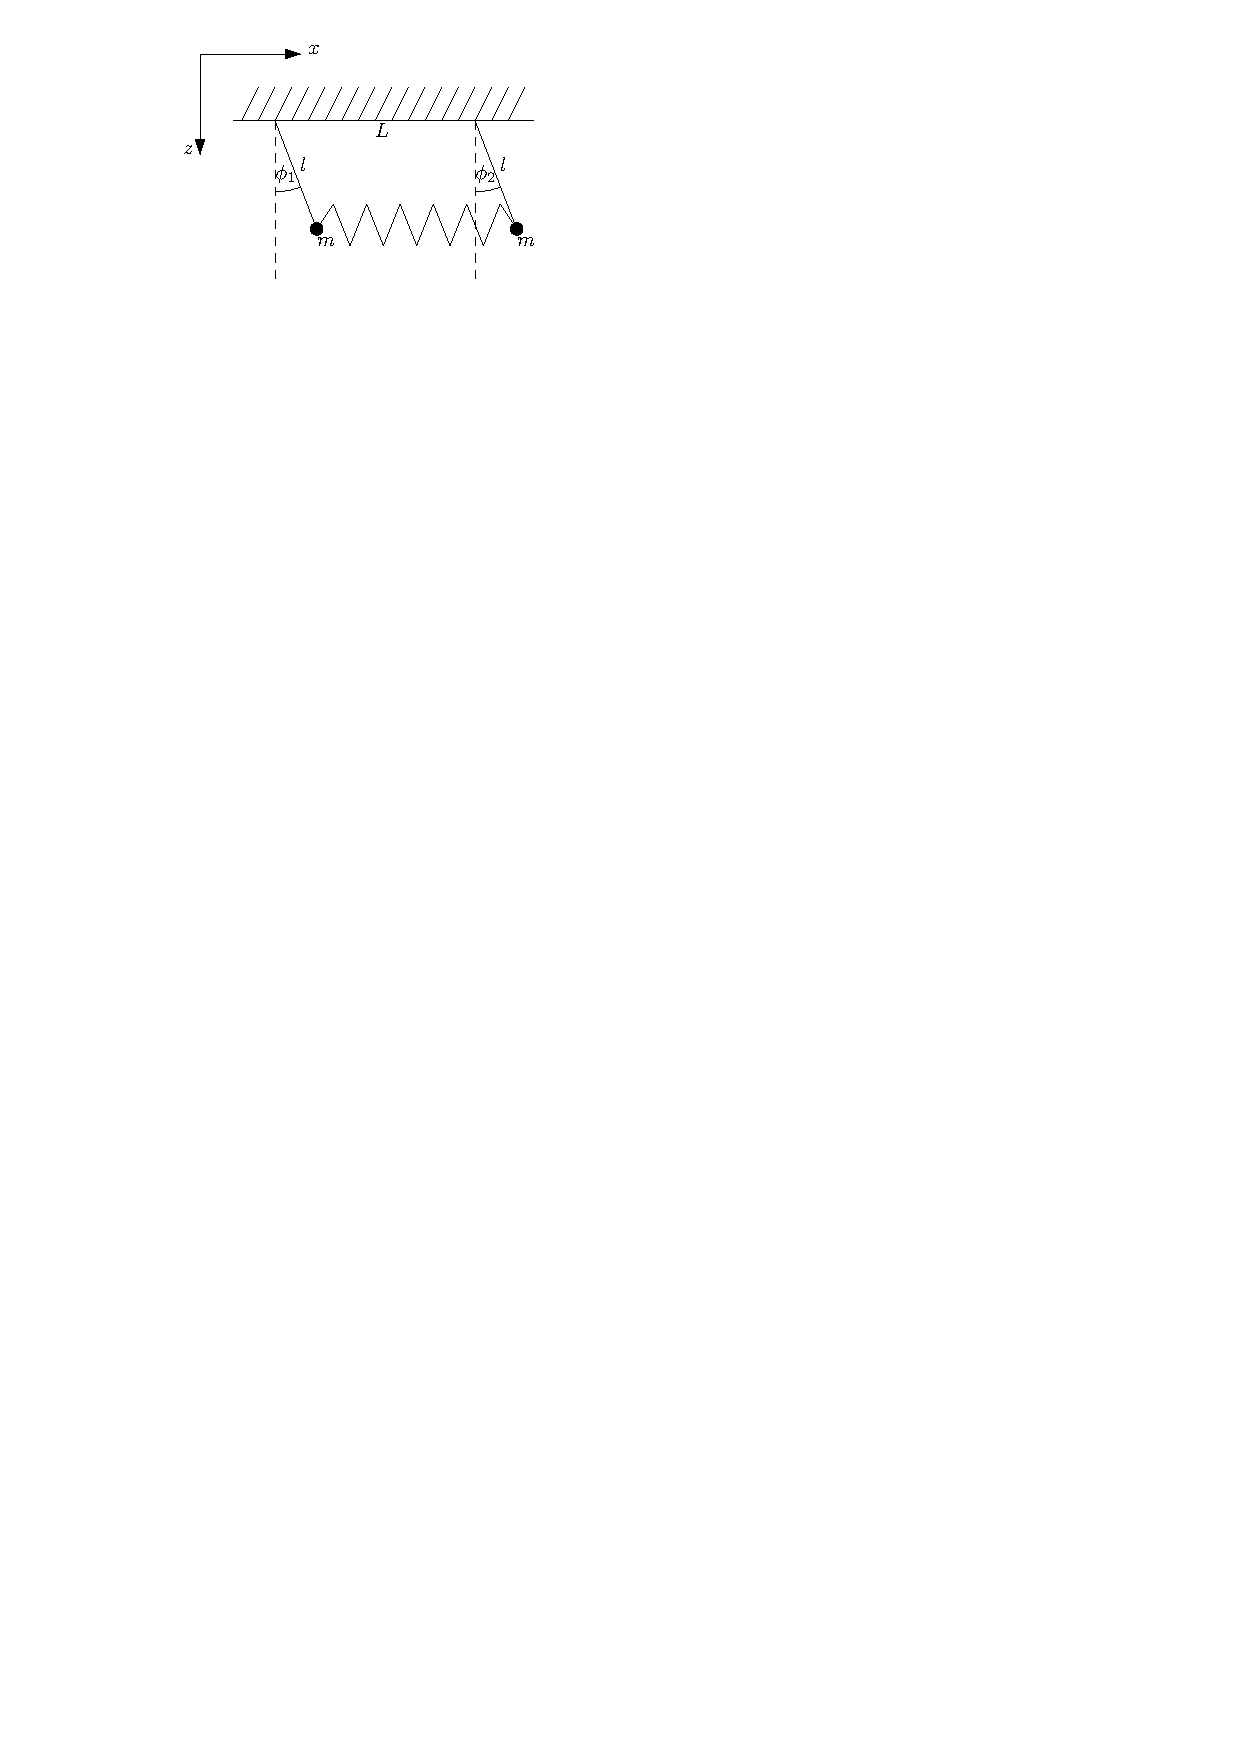
\includegraphics{figures/ueb5/aufgabe12}
	\label{fig:ueb5_aufgabe12}
	\caption{Skizze von Aufgabe 12.}
\end{figure}

Es gilt also:
\[
	x_1 = l \sin \phi_1,
	\quad 
	z_1 = l \cos \phi_1,
	\quad 
	x_2 = l \sin \phi_2 + L
	\quad \text{ und } \quad 
	z_2 = l \cos \phi_2
	\text{.}
\]

Damit folgen die Ableitungen
\begin{align*}
	\dot{x}_1 &= \dot{\phi}_1 l \cos \phi_1, \\
	\dot{x}_2 &= \dot{\phi}_2 l \cos \phi_2, \\
	\dot{z}_1 &= - l \dot{\phi}_1 \sin \phi_1 \text{ und } \\
	\dot{z}_2 &= - l \dot{\phi}_2 \sin \phi_2
	\text{.}
\end{align*}

Die Energien sind
\begin{align*}
	T &= \frac{1}{2} m \left( \dot{x}_1^2 + \dot{z}_1^2 \right)
	+ \frac{1}{2} m \left( \dot{x}_2^2 + \dot{z}_2^2 \right)	
	= \frac{1}{2} m l^2 \left( \dot{\phi}_1^2 + \dot{\phi}_2^2 \right), \\
	V_g &= \sum_{i = 1, 2} - m g z_i = - m g l (\cos \phi_1 + \cos \phi_2) \text{ und } \\
	V_F &= \frac{1}{2} \kappa (x_1 - (x_2 - L))^2 = \frac{1}{2} \kappa l^2 (\sin \phi_1 - \sin \phi_2)^2
\end{align*}
und die Lagrange-Funktion damit
\[
	L = \frac{1}{2} m l^2 (\dot{\phi}_1^2 + \dot{\phi}_2^2)
	- \frac{1}{2} \kappa l^2 (\sin \phi_1 - \sin \phi_2)^2
	+ m g l (\cos \phi_1 + \cos \phi_2)
	\text{.}
\]

Für kleine Auslenkungen approximieren wir mit Taylor:
\begin{align*}
	\sin(x) &= x + \mathcal{O}(x^2) \text{ und } \\
	\cos(x) &= 1 - \frac{x^2}{2} + \mathcal{O}(x^3) = 1 + \mathcal{O}(x^2)
	\text{.}
\end{align*}

Damit vereinfacht sich die Lagrange-Funktion zu
\[
	L = \frac{1}{2} m l^2 (\dot{\phi}_1^2 + \dot{\phi}_2^2)
	- \frac{1}{2} \kappa (\phi_1 - \phi_2)^2
	+ m g l \left( 2 - \frac{\phi_1^2}{2} - \frac{\phi_2^2}{2} \right)
	\text{.}
\]

Jetzt wieder die Lagrange-Gleichungen aufstellen:
\begin{align*}
	\msimplediff{}{t} \frac{\partial L}{\partial \dot{\phi}_1} &= m l^2 \ddot{\phi}_1, \\
	\msimplediff{}{t} \frac{\partial L}{\partial \dot{\phi}_2} &= m l^2 \ddot{\phi}_2, \\
	\frac{\partial L}{\partial \phi_1} &= - \kappa l^2 (\phi_1 - \phi_2) - m g l \phi_1 \text{ und } \\
	\frac{\partial L}{\partial \phi_2} &= \kappa l^2 (\phi_1 - \phi_2) - m g l \phi_2
	\text{.}
\end{align*}

Es folgen daraus die Differentialgleichungen
\[
	\ddot{\phi}_1 = - \frac{\kappa}{m} (\phi_1 - \phi_2) - \frac{g}{l} \phi_1
	\quad \text{ und } \quad 
	\ddot{\phi}_2 = \frac{\kappa}{m} (\phi_1 - \phi_2) - \frac{g}{l} \phi_2
	\text{.}
\]

Mit dem Hinweis:
\begin{align*}
	\ddot{\phi}_2 - \ddot{\phi}_1 &= 2 \frac{\kappa}{m} (\phi_2 - \phi_1) - \frac{g}{l} (\phi_2 - \phi_1), \\
	\underbrace{(\dot{\phi}_2 - \dot{\phi}_1)}_{= \dot{\Phi}_1} &= \left( 2 \frac{\kappa}{m} - \frac{g}{l} \right) \underbrace{\left( \phi_2 - \phi_1 \right)}_{= \Phi_1} \text{ und } \\
	\underbrace{(\dot{\phi}_1 + \dot{\phi}_2)}_{= \dot{\Phi}_2} &= - \frac{g}{l} \underbrace{(\phi_1 + \phi_2)}_{= \Phi_2} \text{.}
\end{align*}

\begin{description}
	\item[Gleichschwingung] $\phi_2 = \phi_1$ $\Longrightarrow$ $\Phi_1 = 0$
	\item[Gegenschwingung] $\phi_2 = -\phi_1$ $\Longrightarrow$ $\Phi_2 = 0$ 
\end{description}

Nun ans Lösen: Wähle den Ansatz 
\[
	\Phi_1(t) = A_1 \cos (\omega_1 t + \beta_1) 
	\quad \text{ und } \quad 
	\Phi_2(t) = A_2 \cos (\omega_2 t + \beta_2)
	\text{.}
\]

Das impliziert $\omega_1^2 = \frac{g}{l} - 2 \frac{\kappa}{m} = \frac{g}{l} \left( 1 - 2 \frac{\kappa}{g} \frac{l}{m} \right)$ und weiter $\omega_2^2 = \frac{g}{l}$. Die anderen Unbekannten bestimmen wir mit den Anfangsbedingungen:
\[
	\phi_1(t = 0) = A
	\quad \text{ und } \quad 
	\phi_2(t = 0) = 0
	\text{.}
\]

Damit $\Phi_1(t = 0) = \phi_1(t = 0) = -A$ und $\Phi_2(t = 0) = - \phi_2(t = 0) = A$. Weiter mit der Anfangsbedingung $\dot{\phi}_1(t = 0) = \dot{\phi}_2(t = 0) = 0$: 
\begin{align*}
	\dot{\Phi}_1(t = 0) &= 0 
	= - A_1 \omega_1 \sin (\omega_1 \cdot 0 + \beta_1) 
	= - A_1 \omega_1 \sin(\beta_1) \text{ und } \\
	\dot{\Phi}_2(t = 0) &= 0 
	= -A_2 \omega_2 \sin(\beta_2) \text{.}
\end{align*}
Also $\beta_1 = \beta_2 = 0$. Zuletzt $\ddot{\Phi}_1(t = 0) = A_1 = A$ und $\ddot{\Phi}_2(t = 0) = A_2 = A$ (wirklich $\ddot{\Phi}$?) 

Am Ende soll folgen: 
\[
	\Phi_1(t) = A \cos (\omega_1 t) 
	\quad \text{ und } \quad 
	\Phi_2(t) = A \cos (\omega_2 t)
	\text{.}
\]

Ergebnis:
\begin{align*}
	\phi_1(t) &= \frac{1}{2} (- \Phi_1 + \Phi_2) = \frac{1}{2} A (\cos(\omega_2 t) - \cos(\omega_1 t)) \text{ und } \\
	\phi_2(t) &= \frac{1}{2} (\Phi_1 + \Phi_2) = \frac{1}{2} A (\cos(\omega_1 t) + \cos (\omega_2 t))
	\text{.}
\end{align*}

Darauf kann man noch die Additionstheoreme $\cos x + \cos y = 2 \cos \left( \frac{x + y}{2} \right) \cos \left( \frac{x - y}{2} \right)$ und $\cos x - \cos y = - 2 \sin \left( \frac{x + y}{2} \right) \sin \left( \frac{x - y}{2} \right)$ anwenden:
\begin{align*}
	\phi_2(t) &= A \cos \left( \frac{\omega_1 + \omega_2}{2} t \right) \cos \left( \frac{\omega_2 - \omega_1}{2} t \right) \\
	\phi_1(t) &= - \underbrace{A \sin \left( \frac{\omega_1 + \omega_2}{2} t \right)}_{= A(t)} \sin \left( \frac{\omega_2 - \omega_1}{2} t \right)
\end{align*}

Interpretation: Die Amplitude ist auch von der Zeit abhängig; wenn die Amplitude von $\phi_2$ am größten ist, ist die Amplitude von $\phi_1$ am kleinsten. Das kann man sich auf \url{http://www.leifiphysik.de/mechanik/kopplung-von-schwingungen/versuche/gekoppelte-pendel-simulation} anschauen.

\end{document}

%%% Local Variables:
%%% mode: latex
%%% TeX-master: t
%%% End:
